\documentclass[border=4pt,12pt]{standalone}
% House style for redrawn exam diagrams (diagram-v4: 0.4pt lines, filled -latex arrows, fine dashes; stipple and hatching drawn as real dots/lines (no PDF/SVG patterns, so they render in every browser and at any scale); transparent background). Every figure \input's this.
\usepackage{amsmath,amssymb}
\usepackage{txfonts}
\usepackage{pdfrender,xcolor}
% \halo{text}: label on shading. The shading stops just around each letter's outline (a thin knock-out that follows the
% glyphs, like the papers' typesetting), never a box. Owner: "I don't want a box around the text".
\newcommand{\halo}[1]{\leavevmode\rlap{\pdfrender{TextRenderingMode=2,LineWidth=2.2pt,LineJoinStyle=1,StrokeColor=white,FillColor=white}#1}#1}
\usepackage{tikz,pgfplots}
\pgfplotsset{compat=1.18}
\usetikzlibrary{arrows.meta,calc,angles,quotes,patterns,patterns.meta,intersections,positioning,decorations.markings,shapes.geometric}
% Stipple and hatching are drawn as actual dots / lines clipped to the region (path picture), NOT as pattern fills:
% SVG <pattern> fills vanish or blur when browsers scale the image, so the owner could not see the shading.
% Each dot is a 0.72pt square (keeps SVGs small; reads as a dot at print size). Dots sit on one global staggered grid, so neighbouring regions line up.
\makeatletter
\newdimen\ex@x \newdimen\ex@y \newdimen\ex@xa \newdimen\ex@ya \newdimen\ex@xb \newdimen\ex@yb \newcount\ex@row
\def\exam@stipplecolor{black!75}\def\exam@dotr{0.42pt}\def\exam@dotgap{2.5}
\def\ex@rowdots{\ifdim\ex@x<\ex@xb \pgfpathrectangle{\pgfqpoint{\dimexpr\ex@x-0.36pt\relax}{\dimexpr\ex@y-0.36pt\relax}}{\pgfqpoint{0.72pt}{0.72pt}}\advance\ex@x by \exam@dotgap pt\relax\expandafter\ex@rowdots\fi}
\def\exam@stipple{%
  \pgftransformreset% dots are sized in real points even inside scaled pictures
  \pgfpointanchor{path picture bounding box}{south west}\ex@xa=\pgf@x \ex@ya=\pgf@y
  \pgfpointanchor{path picture bounding box}{north east}\ex@xb=\pgf@x \ex@yb=\pgf@y
  \pgfsetfillcolor{\exam@stipplecolor}\pgfmathsetmacro\ex@h{\exam@dotgap/2}%
  \pgfmathtruncatemacro\ex@r{floor(\ex@ya/\ex@h)-1}\ex@row=\ex@r\relax
  \ex@y=\ex@r\dimexpr\ex@h pt\relax
  \loop\ifdim\ex@y<\ex@yb
    \pgfmathtruncatemacro\ex@c{floor(\ex@xa/\exam@dotgap)-1}\ex@x=\ex@c\dimexpr\exam@dotgap pt\relax
    \ifodd\ex@row \advance\ex@x by \ex@h pt\fi
    \ex@rowdots
    \advance\ex@y by \ex@h pt \advance\ex@row by 1
    \ifnum\numexpr\ex@row-(\ex@row/4)*4\relax=0 \pgfusepath{fill}\fi% flush every 4 rows: bounded TeX memory, few clip copies in the SVG
  \repeat\pgfusepath{fill}}
\newdimen\ex@d
\def\exam@hatch#1{% #1 = 1 for /, -1 for \ ; lines 45 degrees, 3pt apart
  \pgftransformreset
  \pgfpointanchor{path picture bounding box}{south west}\ex@xa=\pgf@x \ex@ya=\pgf@y
  \pgfpointanchor{path picture bounding box}{north east}\ex@xb=\pgf@x \ex@yb=\pgf@y
  \ex@d=\dimexpr\ex@yb-\ex@ya\relax \ex@x=\dimexpr\ex@xa-\ex@d\relax
  \loop\ifdim\ex@x<\ex@xb
    \ifnum#1>0 \pgfpathmoveto{\pgfqpoint{\ex@x}{\ex@ya}}\pgfpathlineto{\pgfqpoint{\dimexpr\ex@x+\ex@d\relax}{\ex@yb}}%
    \else \pgfpathmoveto{\pgfqpoint{\ex@x}{\ex@yb}}\pgfpathlineto{\pgfqpoint{\dimexpr\ex@x+\ex@d\relax}{\ex@ya}}\fi
    \advance\ex@x by 4.24pt
  \repeat
  \pgfsetlinewidth{0.4pt}\pgfsetstrokecolor{black}\pgfusepath{stroke}}
\def\examstipple{\exam@stipple}\def\examhatch{\exam@hatch}\def\examsetstipplecolor#1{\def\exam@stipplecolor{#1}}\def\examsetdotgap#1{\def\exam@dotgap{#1}}
\makeatother
% (legacy pattern kept for old files)
% staggered stipple like the NESA papers' dotted shading
\pgfdeclarepatternformonly{exam stipple}{\pgfpointorigin}{\pgfqpoint{2.2pt}{2.2pt}}{\pgfqpoint{2.2pt}{2.2pt}}{%
  \pgfpathcircle{\pgfqpoint{0.55pt}{0.55pt}}{0.42pt}\pgfpathcircle{\pgfqpoint{1.65pt}{1.65pt}}{0.42pt}\pgfusepath{fill}}
\tikzset{
  every picture/.style={line width=0.6pt, >={Latex[length=2mm,width=1.3mm]}},
  curve/.style={line width=0.6pt},
  open arrow/.style={-{Latex[length=2mm,width=1.3mm]}},  % owner: filled -latex heads everywhere, no open chevrons
  aux/.style={dash pattern=on 2pt off 1.5pt, line width=0.6pt},
  shade/.code={\def\exA{#1}\def\exB{none}\ifx\exA\exB\else\pgfkeysalso{fill=black!18}\fi},
  shade/.default=on,
  shade dots/.style={fill=none, path picture={\examstipple}},
  stipple color/.code={\examsetstipplecolor{#1}},
  stipple gap/.code={\examsetdotgap{#1}},
  shade dense dots/.style={fill=none, stipple gap=1.6, path picture={\examstipple}},
  shade hatch/.style={fill=none, path picture={\examhatch{1}}},
  shade hatch reverse/.style={fill=none, path picture={\examhatch{-1}}},
  shade solid/.style={fill=black},
  pt/.style={circle, fill, inner sep=1.1pt},
  open pt/.style={circle, draw, fill=white, inner sep=1.1pt},
}
\pgfplotsset{
  exam axes/.style={axis lines=middle, axis line style={->}, xlabel={$x$}, ylabel={$y$},
    xlabel style={anchor=west}, ylabel style={anchor=south}, tick label style={font=\small},
    every axis plot/.append style={line width=0.6pt, black}, samples=200, clip=false,
    enlargelimits=false, axis on top},
}

\begin{document}
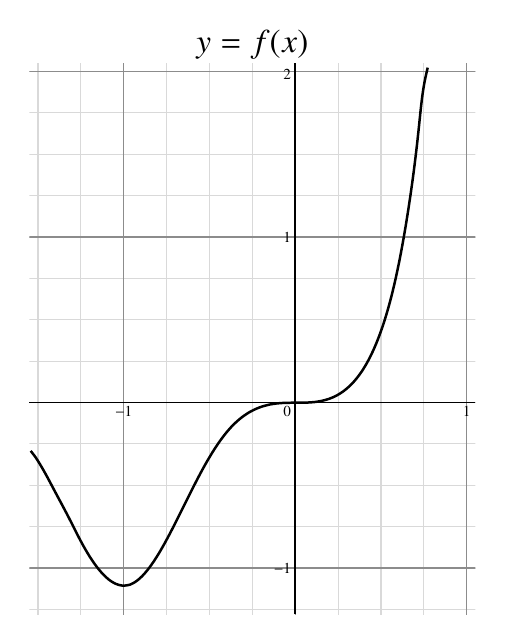
\begin{tikzpicture}[x=2.1780cm,y=2.1018cm]
  % Desmos-style grid: minor lines every 0.25, major every 1 (light grey), axes black, no arrowheads (as the crop)
  \begin{scope}
  \clip (-1.55,-1.28) rectangle (1.05,2.05);
  \draw[black!15,line width=0.4pt] (-1.75,-1.5) grid[step=0.25] (1.25,2.25);
  \draw[black!45,line width=0.5pt] (-2,-2) grid[step=1] (2,3);
  \end{scope}
  \draw (-1.55,0) -- (1.05,0); \draw (0,-1.28) -- (0,2.05);
  \tikzset{tl/.style={font=\fontsize{5.5}{6}\selectfont,inner sep=1.2pt}}
  \node[tl,below] at (-1,0) {$-1$}; \node[tl,below] at (1,0) {$1$}; \node[tl,below left] at (0,0) {$0$};
  \node[tl,left] at (0,1) {$1$}; \node[tl,below left] at (0,2.04) {$2$}; \node[tl,left] at (0,-1) {$-1$};
  % curve traced from the crop (unknown function), fitted as a smoothing spline y(x) (column centres of the stroke)
  \begin{scope}
  \clip (-1.56,-1.29) rectangle (1.06,2.06);
  \draw[line width=0.9pt] plot[smooth] coordinates {(-1.5423,-0.2919) (-1.5156,-0.3283) (-1.4916,-0.3667) (-1.4692,-0.4061) (-1.4478,-0.4460) (-1.4270,-0.4863) (-1.4064,-0.5267) (-1.3857,-0.5671) (-1.3648,-0.6074) (-1.3441,-0.6478) (-1.3236,-0.6883) (-1.3036,-0.7290) (-1.2838,-0.7699) (-1.2638,-0.8106) (-1.2431,-0.8510) (-1.2215,-0.8909) (-1.1987,-0.9300) (-1.1743,-0.9681) (-1.1479,-1.0047) (-1.1189,-1.0392) (-1.0864,-1.0700) (-1.0491,-1.0942) (-1.0068,-1.1063) (-0.9634,-1.1003) (-0.9248,-1.0783) (-0.8918,-1.0481) (-0.8627,-1.0138) (-0.8363,-0.9772) (-0.8118,-0.9391) (-0.7887,-0.9002) (-0.7667,-0.8605) (-0.7455,-0.8205) (-0.7249,-0.7800) (-0.7047,-0.7394) (-0.6848,-0.6986) (-0.6651,-0.6577) (-0.6454,-0.6167) (-0.6258,-0.5758) (-0.6061,-0.5349) (-0.5861,-0.4941) (-0.5659,-0.4535) (-0.5452,-0.4131) (-0.5239,-0.3731) (-0.5018,-0.3335) (-0.4788,-0.2944) (-0.4548,-0.2561) (-0.4294,-0.2187) (-0.4024,-0.1826) (-0.3735,-0.1481) (-0.3421,-0.1159) (-0.3082,-0.0866) (-0.2717,-0.0610) (-0.2327,-0.0398) (-0.1915,-0.0234) (-0.1488,-0.0119) (-0.1052,-0.0050) (-0.0612,-0.0018) (-0.0171,-0.0010) (0.0270,-0.0009) (0.0711,0.0000) (0.1151,0.0035) (0.1586,0.0110) (0.2009,0.0238) (0.2412,0.0423) (0.2786,0.0665) (0.3127,0.0954) (0.3435,0.1281) (0.3713,0.1636) (0.3963,0.2013) (0.4189,0.2405) (0.4394,0.2810) (0.4582,0.3224) (0.4754,0.3645) (0.4914,0.4071) (0.5063,0.4501) (0.5202,0.4935) (0.5331,0.5372) (0.5453,0.5812) (0.5568,0.6253) (0.5676,0.6696) (0.5779,0.7141) (0.5876,0.7587) (0.5969,0.8034) (0.6058,0.8482) (0.6143,0.8930) (0.6224,0.9380) (0.6303,0.9830) (0.6378,1.0280) (0.6452,1.0731) (0.6522,1.1182) (0.6591,1.1634) (0.6657,1.2086) (0.6722,1.2538) (0.6784,1.2991) (0.6845,1.3444) (0.6903,1.3897) (0.6959,1.4350) (0.7013,1.4804) (0.7065,1.5258) (0.7115,1.5712) (0.7163,1.6167) (0.7210,1.6622) (0.7255,1.7076) (0.7300,1.7531) (0.7348,1.7986) (0.7401,1.8440) (0.7463,1.8892) (0.7537,1.9343) (0.7626,1.9791) (0.7726,2.0236)};
  \end{scope}
  \node[anchor=south,inner sep=1pt,font=\large] at (-0.25,2.05) {$y=f(x)$};
\end{tikzpicture}
\end{document}
